\section{Finanzierung und Sponsoren von Open Source}

% Einleitung
Ein weiterer Faktor, der Nutzer davon überzeugen kann ein gewisses Framework oder Bibliothek 
gegenüber einer anderen zu nutze, ist die finanzielle Sicherheit eines Projekts. Es wird vermutet,
dass Projekte mit Sponsoren beliebter bei Nutzer sind als Projekte ohne.
Die Information, ob ein Projekt Sponsoren hat ist für einen neuen potenziellen Nutzer hierbei in der
Regel sehr leicht ersichtlich. 
VueJS beispielsweise macht sowohl auf der Website als auch in der README.md auf die Sponsoren aufmerksam
und bedankt sich für ihre Unterstützung, wie in Abbildung \ref{abb:VueJS_Sponsors} zu erkennen ist.

Daraus ergibt sich die erste Hypothese,

\begin{hypothesis}
    Sponsoren haben einen positiven Einfluss bei der Auswahl von OSS auf die Nutzer, demnach haben
    gesponserte Projekte einen höheren Markterfolg.   
\end{hypothesis}

Außerdem kann durch die finanzielle Unterstützung der Sponsoren die Produktivität gefördert werden.
Das Projekt wird schneller weiter entwickelt und sorgfältiger gewartet. Daraus ergibt sich die 
zweite Hypothese bezüglich Sponsoren:

\begin{hypothesis}
    Gesponserte Projekte haben einen höheren technischen Erfolg
\end{hypothesis}

\begin{figure}[h]
    \centering
    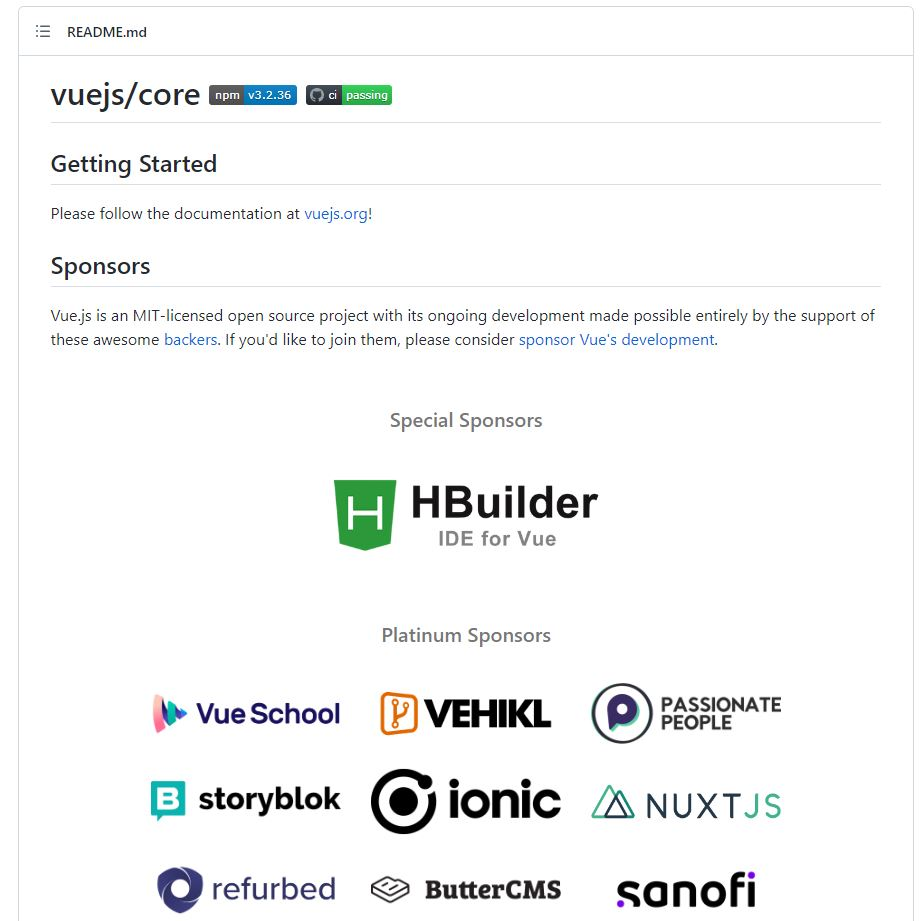
\includegraphics[scale=0.6]{figures/02/VueSponsoren.JPG}
    \caption{VueJS Top Sponsoren}
    \label{abb:VueJS_Sponsors}
\end{figure}
